\providecommand{\main}{../../..}
\providecommand{\Figures}{\main/Figures}

\documentclass[\main/main.tex]{subfiles}

\begin{document}

\chapter{
    \label{sec:montage}
    Méthode 1 : Uniformiser le montage permet de simplifier et d'accélérer l'acquisition des échantillons
    }

\chaptermark{Uniformiser le montage pour accélérer l'acquisition}

    \section{L'impression 3D permet de créer rapidement et simplement des solutions de montage peu onéreuses}
    
%%
%
Grâce aux avantages présentés dans la section~\ref{sec:lempereur_bio}, le développement de l'impression 3D a permis l'émergence d'un grand nombre de techniques.
%
Pour le grand public, la crise actuelle du coronavirus a démontré l'intérêt de l'impression 3D
pour des projet simples, comme la production de protections ou de raccord de matériels médicaux~\cite{callahan_2020,ishack_2020,wesemann_2020}, comme pour des projets plus complexes, comme la création de respirateurs artificiels ou de pousse-seringues open-sources~\cite{na_website_nda}.
%
Cette crise a ainsi montré la rapidité et l'adaptabilité de l'impression 3D.
%
Mais la communauté scientifique avait déjà intégrée cette technologie pour le prototypage~\cite{he_2016}, la normalisation d'expérience ~\cite{pinskiy_2013} ou encore l'éducation~\cite{maiachagas_2017}.
    
%%
%
L'acquisition automatique des échantillons nécessité la mise en place de procédure simples
et reproductibles permettant de placer les échantillons.
%
Différentes procédures de montages ont été publiées ces dernières années.
%
Le choix de l'impression 3D est apparu naturellement, car cette technologie permet de coupler versatilité, simplicité et reproductibilité.
%
Dans le cadre de l'acquisition automatique, les projets les plus intéressants consistent en la création de tampons comportant des encoches.
%
L'impression de ces tampons dans un support comme de l'agarose ou du picodent( pâte dentaire) permet tout d'abord de créer un système de coordonnées précis
permettant de simplifier l'automatisation de l'acquisition. En effet, la précision de l'impression 3D permet de définir précisément l'espacement entre deux échantillons.
Il est ainsi possible de paramétrer des acquisitions multiples en renseignant la position du premier échantillon puis les distances entre les échantillons.
%%
%
Un second avantage est la création d'un guide pour faciliter les montage. Dans la plupart des cas, le montage des échantillons dos vers le haut (vue dorsale)
est le plus favorable à l'acquisition d'échantillons entiers. En vue latérale,le cristallin et la rétine interfèrent avec la diffusion de la lumière au sein des tissus et mènent à des images inappropriées.
Dans le cas d'acquisitions ventrales, la forte quantité de protéines et de lipides se trouvant dans le sac vitellin empêche l'acquisition au travers de ce tissu.
%
L'utilisation d'un tampon dédié va permettre de créer des encoches ayant une forme spécifiquement destinée à favoriser le montage dos vers le haut.

%% Plaque 96
%
Une première publication notable dans l'emploi de l'impression 3D pour le montage d'échantillon de \pz{} utilisait des plaques 96 puits~\cite{wittbrodt_2014}.
%
Il s'agissait d'imprimer deux parties distinctes.%
%
La première partie, qui doit être imprimé six fois, consiste en une ligne présentant des projections.
%
Ces projections servent à imprimer dans chaque puits de la plaque une encoche dans de l'agarose.
%
Deux formes d'encoches sont proposées, une première permettant le montage en latéral quand seconde forme permet le montage en position dorsale.
%
La seconde partie à imprimer est un cadre afin d'assurer l'espacement entre les lignes.
%
Ce processus permet de placer les échantillons précisément au centre des puits d'une plaque 96 puits tout en simplifiant l'orientation de ces échantillons.
%
Malheureusement, Cette méthode présente l'inconvénient de ne pouvoir effectuer des images avec des objectifs plongeants à haut indice de réfraction, leur diamètre étant trop grand pour que les bords des puits n'entraîne pas d'abération.
%
Une seconde publication propose l'utilisation de cadres imprimés en 3D permettant de monter les échantillons entre deux lamelles~\cite{alessandri_2017}.
%
Dans cette publication, trois parties sont imprimées.
%
La première est un cadre servant de réceptacle pour une première lamelle en verre et un cadre en polydiméthylsiloxane. La lamelle sert de support à une feuille d'agarose.
Le cadre en polydiméthylsiloxane sert de joint.
%
La seconde partie est un tampon permettant la création de niches circulaires au sein de la feuille d'agarose.
%
Ces niches vont ensuite accueillir des oeufs de \pz{}.
%
Une fois les oeufs placés dans les niches, la feuille d'agarose est recouverte d'une seconde lamelle en verre.
%
Enfin, la dernière partie imprimée est un couvercle permettant de sceller l'ensemble.
%
Cette stratégie permet de réaliser le montage d'une grande quantité d'échantillons de petite taille, comme des oeufs de \pz{}.
%
L'ensemble étant scellé, il est ainsi possible d'imager l'ensemble avec un montage microscopique droit comme un montage inversé.
%
Cependant, la petite taille de la lamelle empêche d'imager des stades tardifs, et la création d'un ensemble scellé empêche l'emploi d'objectifs plongeants.

%%
Enfin, la publication de Kleinhans et Lecauday en 2019 propose l'impression d'un tampon permettant d'imprimer des encoches dans de l'agarose placé au fond d'une boite de Petri~\cite{kleinhans_2019}.
%
Ce tampon permet le montage en latéral de larves de \pz entre 22 et 96 hpf.
%
Une fois le tampon imprimé, il est placé sur une tête de vis afin de pouvoir manipuler plus facilement l'ensemble.
%
Cette approche est comparable à celle que j'ai développé au cours de ma thèse, mais j'ai procédéà plusieurs optimisations.
%
Elle a pour avantage d'être compatible avec l'utilisation d'objectifs à lentille plongeante, car elle permet de créer des espaces vides autour de la zone d'acquisitions.
%
De plus, Il est possible de facilement adapter la forme de la base à différents types de supports, que ce soit des boites de Petri ou des boites de cultures cellulaires.
%
En revanche, la présence d'une couche d'agarose entre le fond du support de montage et l'échantillon rend l'utilisation de cette solution incompatible avec un montage microscopique inversé.

%%
% 
Dans le cadre de la publication présentée en section~\ref{sec:lempereur_bio},
nous avons proposé des tampons permettant de monter 12 ou 48 \pzs{} à 5 dpf 
(voir Figure~\ref{fig:tampon} et Figure~\ref{fig:formes:whole_5dpf}).
%
Au cours de ma thèse, d'autres modèles de tampons ont été développés afin de tester la versatilité de notre approche tout en répondant aux demandes variées des utilisateurs de TPS.
%
Ainsi, le tampon créé pour des \pzs{} à 5 dpf a été utilisé pour monter des \pzs{} entre 3 et 10 dpf.
%
Pour monter des \pzs{} plus âgés, deux tampons ont été créés, ce qui permet de
couvrir l'ensemble des stades entre 3 et 21 dpf.
%
De plus, des formes spécifiques ont été développées pour permettre le montage d'échantillons
d' \ol{}, ou pour permettre le montage de cerveaux de \pz{} à 21 dpf et 6 wpf
(voir Figure~\ref{fig:formes:brain_21dpf} et \ref{fig:formes:brain_6wpf}).

\begin{figure}[htbp]
    \centering
    \begin{subfigure}[b]{0.57\textwidth}
       \caption{
            \label{fig:tampon:12}
            12 échantillons
            }
       \centering 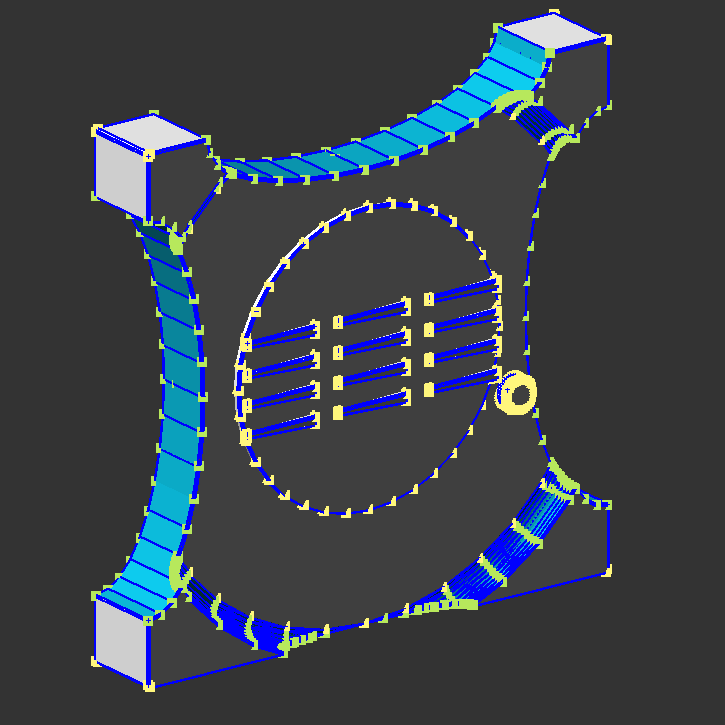
\includegraphics[width=\textwidth]{\Figures/Moules/whole_12_cut.png}
    \end{subfigure}
    \begin{subfigure}[b]{0.38\textwidth}
       \caption{
        \label{fig:tampon:48}
        48 échantillons
        }
       \centering 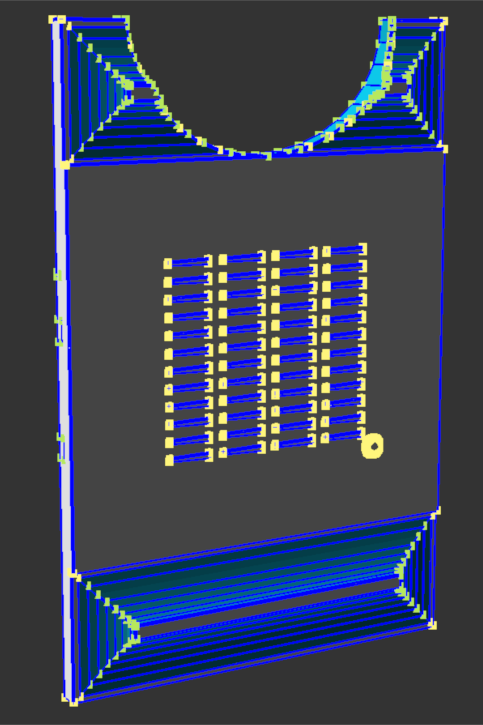
\includegraphics[width=\textwidth]{\Figures/Moules/whole_48_cut.png}
    \end{subfigure}
    \caption{
        \label{fig:tampon}
        Représentations surfaciques de moules permettant le montage de 12 ou 48 alevins de \pzs{}.
        Ces moules permettent d'assurer un espacement régulier entre les échantillons.
    }
    
\end{figure}

\begin{figure}[htbp]
    \centering
    \begin{subfigure}[b]{0.37674418604651162790697674418605\textwidth}
       \caption{
            \label{fig:formes:whole_5dpf}
            échantillon entier à 5 dpf
            }
       \centering \includegraphics[width=\textwidth]{\Figures/Moules/whole_5dpf_cut.png}
    \end{subfigure}
    \begin{subfigure}[b]{0.26162790697674418604651162790698\textwidth}
       \caption{
            \label{fig:formes:brain_21dpf}
            Cerveau à 21 dpf
            }
       \centering 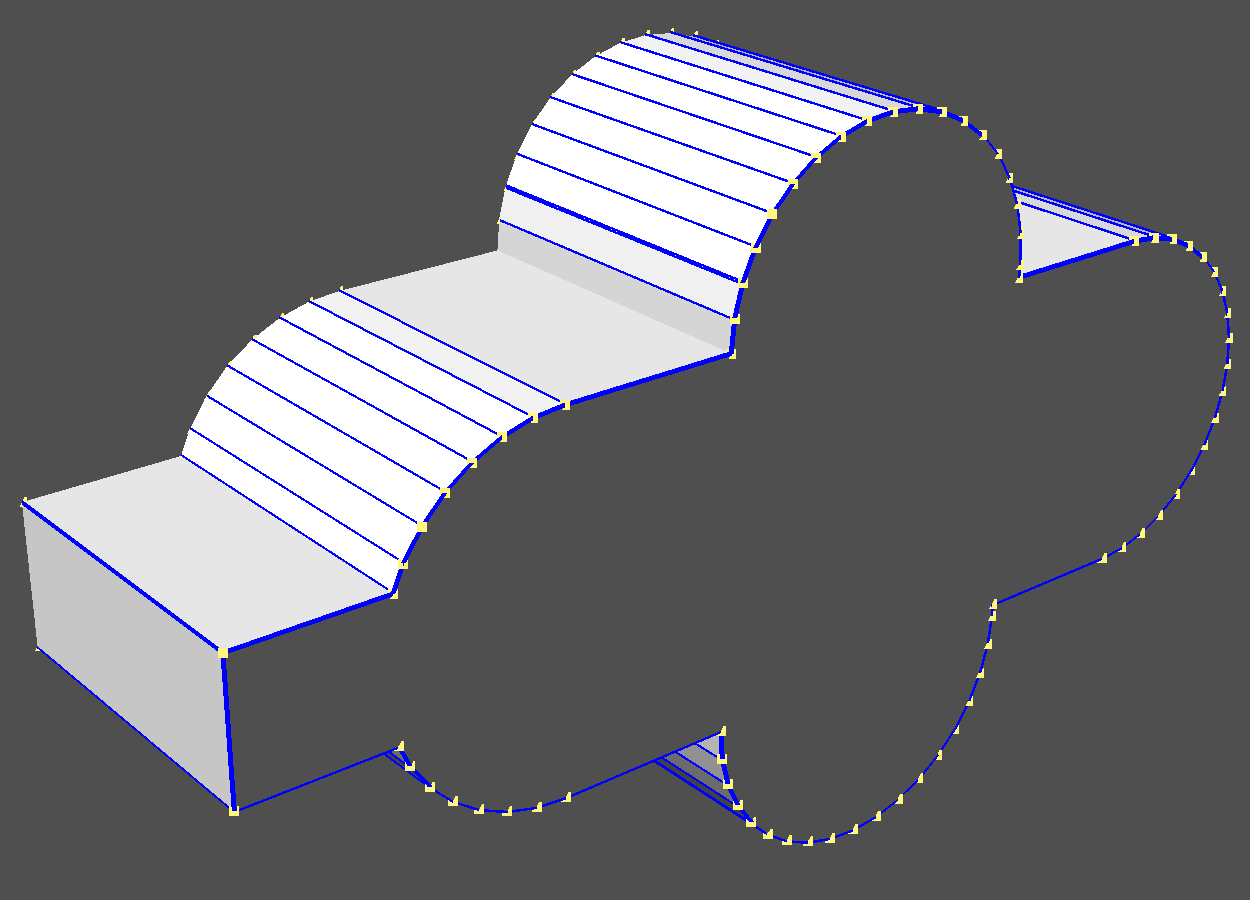
\includegraphics[width=\textwidth]{\Figures/Moules/brain_21dpf_cut.png}
    \end{subfigure}
    \begin{subfigure}[b]{0.26162790697674418604651162790698\textwidth}
       \caption{
            \label{fig:formes:brain_6wpf}
            Cerveau à 6 wpf
            }
       \centering 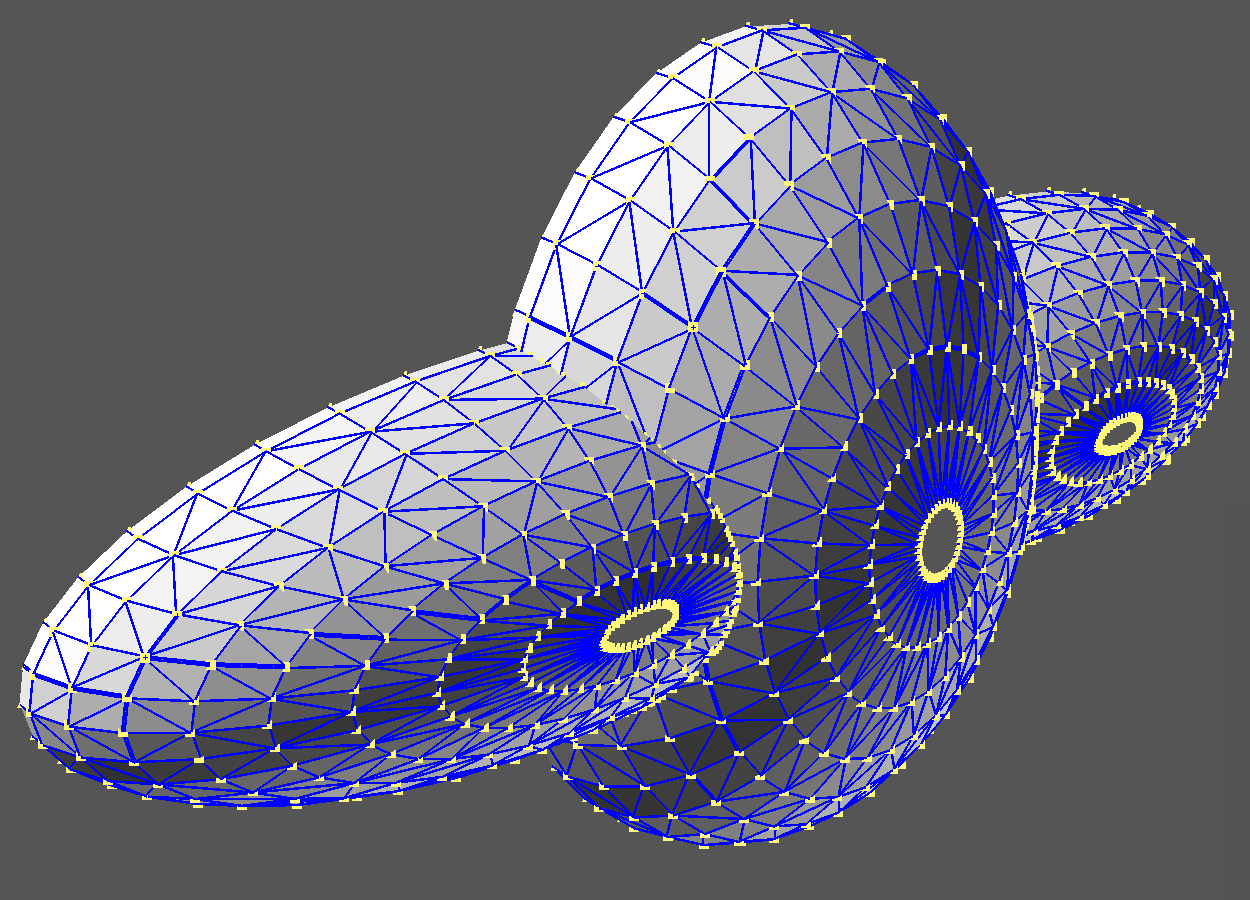
\includegraphics[width=\textwidth]{\Figures/Moules/brain_6wpf_cut.png}
    \end{subfigure}
    \caption{
        \label{fig:formes}
        Représentations surfaciques des encoches permettant le montage de \pzs. Ces encoches permettent ainsi de s'adapter à différents stades de développement ou permettent de monter un organe disséqué comme le cerveau.
    }
    
\end{figure}
    
    \section{Plusieurs approches infructueuses ont été développées avant d'utiliser l'impression 3D}
 
%%
%
La méthode de montage présentée dans le cadre de cette thèse et ses dérivés se base sur la version la plus aboutie des moules.
%
Dans cette section, nous allons faire une rétrospective des approches de montage envisagées, en présentant quelles étaient les perspectives offertes par chaque approche, ainsi que les raisons ayant mené à l'abandon de ces approches.

%%
%
La première approche développée consistait simplement en l'impression d'une grille type papier millimétrée placée sous le fond d'une boite de Petri, afin d'aligner le mieux possible les échantillons.
%
Une fois les échantillons placés sur la plaque, ils étaient recouvert d'une goutte d'agarose ou de phytagel afin de les stabiliser.
%
Cette technique présente de nombreux défauts. Tout d'abord, la qualité d'orientation des échantillons est très mauvaise, et dépend pour beaucoup de l'opérateur.
%
Ensuite, bien que l'utilisation d'une grille permette un positionnement visuellement bon, l'imprécision générée par cette méthode était incompatible avec les nécessités de l'imagerie par microscopie confocale.
%
Enfin, la mise en place de la goutte d'agarose amplifiait les problèmes précédents, car la larve n'étant pas correctement maintenue en place, il était fréquent que la larve se déplace une fois la goutte d'agarose déposée.
%
Cette méthode nécessitait un compromis important entre vitesse et qualité de montage.
%
Malgré tout, cette approche a été conservée pour le montage d'échantillons ayant des formes adaptées, comme les coupes épaisses de tissus cérébraux murins.
%
De plus, il s'agit actuellement de la seule méthode permettant d'effectuer l'acquisition d'un même échantillon via un objectif à lentille plongeante et via un montage destiné à un microscope inversé.
%
Une seconde approche consistait en l'utilisation de deux parties usinées.
%
La première partie était simplement une cuve en aluminium comportant des filetages.
%
C'est sur cette plaque que les échantillons à imager devaient être fixés par une goutte d'agarose.
%
L'aluminium a été choisi afin de favoriser l'adhérence, afin de pouvoir s'assurer de la planéarité de la zone d'acquisition et pour servir de réceptacle étanche et sans risque pour les échantillons.
%
Les filetages servaient à aligner précisément la seconde partie dans cette cuve, et permettait d'améliorer l'étanchéité entre les deux parties.
%
La seconde partie consistait en une plaque de Teflon possédant des fentes, ainsi que des trous en opposition au filetages de la cuve en aluminium.
%
Le choix du Teflon a été fait car il s'agit d'un matériaux dont l'adhérence est minimale.
%
La distance entre les fentes a été choisie afin de permettre de charger la plaque via l'utilisation d'un micro-pipette multi-canaux.
%
Ainsi, la plaque en Téflon devait à la fois servir de guide pour le placement des échantillons, puis de cage pour empêcher le déplacement des échantillons lors de l'ajoût de l'agarose.
%
L'agarose aurait alors adhéré à la plaque en aluminium.
%
Cette stratégie a été abandonnée car il était impossible de faire adhérer les échantillons sur le fond de la cuve d'acquisition tout en s'assurant de leur positionnement.
%
En effet, l'agarose se fixait réguliérement dans les fentes de la plaque en Teflon lorsque l'étanchéité entre les deux plaques étaient fortes, mais les échantillons passaient entre les deux parties si cette étanchéité était réduite.
%
Plusieurs tentatives de modifications ont été effectuées, comme l'inclusion d'un grillage fixé au fond de la cuve en aluminium permettant de faciliter l'adhérence, ou encore l'addition d'une troisième plaque pour permettre à l'agarose de ne pas rester dans les fentes de la plaque en Teflon, mais aucune des modifications effectuées ne fut en mesure de permettre de rendre cette approche praticable.
%
Notre dernière approche fut l'emploi de l'impression 3D comme décrit précédemment.
%
Cherchant à imprimer des pièces ayant une précision de l'ordre de la centaine de micromètres, une optimisation des méthodes d'impressions a été nécessaire. 

    \section{L'optimisation des paramètres et des conditions d'impression est nécessaire à des impressions 3D reproductibles}

%%
%
Avec les technologies à budget de moyenne gamme dont nous disposions au laboratoire, l'impression 3D présentait de nombreuses limitations pour la création de d'objets précis. Dans les chapitres suivants, je décris un certain nombre d'optimisations que j'ai réalisé afin de contribuer à la pérennité de cette technologie au sein de la plateforme.
%
Une première limitation était la taille de la buse, qui empêchait la création d'objets présentant des parties minces.
%
En effet, l'emploi d'une buse d'impression ayant un diamètre de 0.25 mm ne permet pas l'impression d'éléments ayant une taille inférieure à 0.30 mm, à cause de l'étalement de la matière autour du lieu de dépôt. Les puits pour des larves à 5 dpf possédant une taille de 0,25mm dans la région caudale risquaient donc d'être insuffisamment précisément imprimés.
%
Nous avons résolu ce problème en imprimant les régions d'intérêt non plus à l'horizontale mais à la verticale (voir Figure~\ref{fig:coupe:model:horizontal} et \ref{fig:coupe:model:vertical}). Comme l'épaisseur minimale d'une couche est de 60 µm en utilisant la même buse de 0.25 mm, il devenait possible de créer des formes possédant la taille désirée avec une précision suffisante.
%
Une ligne de quelques centaines de micromètres devient alors une surface complexe ayant toujours une épaisseur supérieure à la taille limite de 60 µm  (voir Figure~\ref{fig:coupe:slicing:horizontal} et \ref{fig:coupe:slicing:vertical}).
%
Ainsi, j'ai pu imprimer des éléments plus fins (voir Figure~\ref{fig:coupe:comp:horizontal} et \ref{fig:coupe:comp:vertical}).

\begin{figure}[h!]
    \centering
    \begin{subfigure}[b]{0.45\textwidth}
       \centering \caption{
            \label{fig:coupe:model:horizontal}
            Vue de dessus du modèle théorique
            }
       \centering 
\includegraphics[width=\textwidth]{\Figures/Moules/modele_horizontal.png}
    \end{subfigure}
    \begin{subfigure}[b]{0.45\textwidth}
       \centering \caption{
            \label{fig:coupe:model:vertical}
            Vue de coté du modèle théorique
            }
       \centering 
\includegraphics[width=\textwidth]{\Figures/Moules/modele_vertical.png}
    \end{subfigure}
    \begin{subfigure}[b]{0.45\textwidth}
       \centering \caption{
            \label{fig:coupe:slicing:horizontal}
            Vue de dessus des consignes
            }
       \centering 
\includegraphics[width=\textwidth]{\Figures/Moules/consigne_horizontal.png}
    \end{subfigure}
    \begin{subfigure}[b]{0.45\textwidth}
       \centering \caption{
            \label{fig:coupe:slicing:vertical}
            Vue de coté des consignes
            }
       \centering 
\includegraphics[width=\textwidth]{\Figures/Moules/consigne_vertical.png}
    \end{subfigure}
    \begin{subfigure}[b]{0.45\textwidth}
       \centering \caption{
            \label{fig:coupe:comp:horizontal}
            Comparaison entre les consignes et le modèle théorique pour une vue de dessus
            }
       \centering 
\includegraphics[width=\textwidth]{\Figures/Moules/comp_horizontal.png}
    \end{subfigure}
    \begin{subfigure}[b]{0.45\textwidth}
       \centering \caption{
            \label{fig:coupe:comp:vertical}
            Comparaison entre les consignes et le modèle théorique pour une vue de coté
            }
       \centering 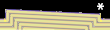
\includegraphics[width=\textwidth]{\Figures/Moules/comp_vertical.png}
    \end{subfigure}
    
    \caption{
        \label{fig:coupe}
        L'impression des tampons à la verticale permet de profiter au mieux de la précision permise par l'impression 3D (taille minimale d'impression : 250 $\mu$m à l'horizontal contre 60 $\mu$m à la verticale).
        \newline
        Le modèle théorique (a;b) est issu du logiciel de conception 3D \href{https://www.openscad.org/}{openscad}.
        Le logiciel de découpe de modèle 3D \href{https://ultimaker.com/fr/software/ultimaker-cura}{Cura 4} permet de traduire le modèle théorique en consigne pour l'impression (c;d) en découpant le modèle en couche que l'imprimante sera capable de déposer.
        Le comparaison entre le modèle théorique et la consigne obtenue montre des différences importantes si le tampon est imprimé à l'horizontal, différences qui seront amplifiées lors de l'impression (e;f).
        En particulier, les parties fines prévues pour accueillir la queue de l'EE (astérisque) ne pourront pas être correctement imprimées.
    }
    
\end{figure}

%%
%
Malheureusement, en position verticale, lorsque l'impression est orientée orthogonalement à la grande longueur de la plaque, les forces de cisaillement lors des aller-retours très rapides de la buse entraînaient des cassures de la plaque aléatoires lors de l'impression.
%
Une première stratégie pour résoudre ce problème a été de réduire la vitesse de déplacement de la buse afin de limiter l'impact des déplacements. Cependant, ce réglage s'est révélé insuffisant.
%
Une seconde stratégie a tiré parti du mode d'impression. En effet, Cura produit des fichiers dont l'impression des parties internes de l'objet se fait en diagonale par rapport au plateau de l'imprimante (voir Figure~\ref{fig:print:axe}).
Ainsi, afin de permettre de réduire par deux les à-coups, les pièces à imprimer ont été placées de manière à ce que leur plus grande longueur se situe dans la diagonale du plateau d'impression (voir Figure~\ref{fig:print:diag}).
%%
%
Par ailleurs, l'impression 3D est sensible aux conditions de température ou de flux d'air du local où l'impression est effectuée. Les courants d'air induisaient des défauts aléatoire, surtout avec les pièces fines. Afin de pallier ce problème, certaines imprimantes 3D (pas l'Ultimaker 2 disponible au laboratoire), possèdent une enceinte fermée, ce qui permet de mieux contrôler la température au sein de cette enceinte. 
J'ai pu compenser ce problème par l'impression d'une enceinte pare-brise, option permise par le logiciel de découpe par tranche Cura 4.
%(voir Figure~\ref{fig:print:shield}.
%
De cette manière, une enceinte va se créer autour de l'objet à imprimer, permettant de réduire les risques de courants d'air tout en permettant de maintenir plus facilement une température homogène dans cette enceinte. Cette solution ne permet cependant pas de s'abstenir de protéger complètement l'imprimante contre les courants d'airs, mais constitue une solution d'appoint pour limiter leur impact.



\begin{figure}[htbp]
    \centering
    \begin{subfigure}[b]{0.30\textwidth}
       \centering \caption{
            \label{fig:print:axe}
            Consignes d'impression pour un objet placé en diagonale de l'axe d'impression
            }
       \centering 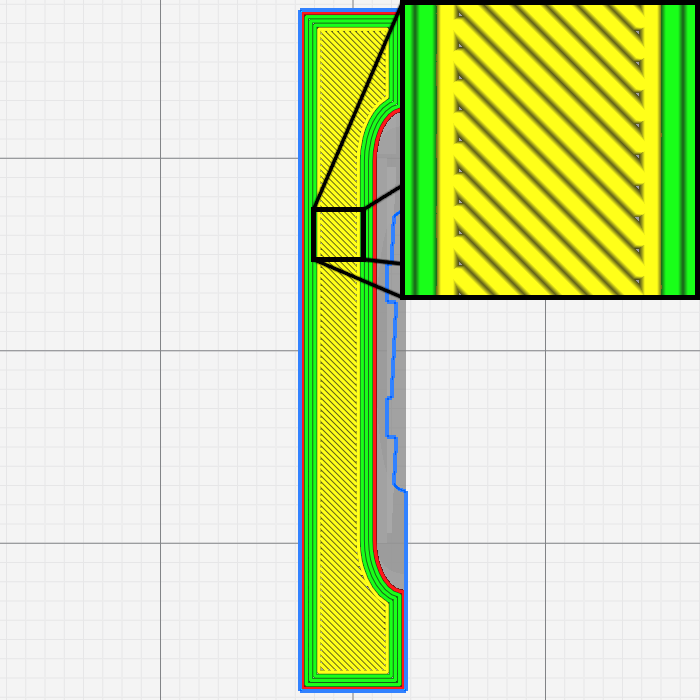
\includegraphics[width=\textwidth]{\Figures/Moules/coupe_axe_zoom.png}
    \end{subfigure}
    \begin{subfigure}[b]{0.30\textwidth}
       \centering \caption{
            \label{fig:print:diag}
            Consignes d'impression pour une objet placé dans l'axe d'impression
            }
       \centering 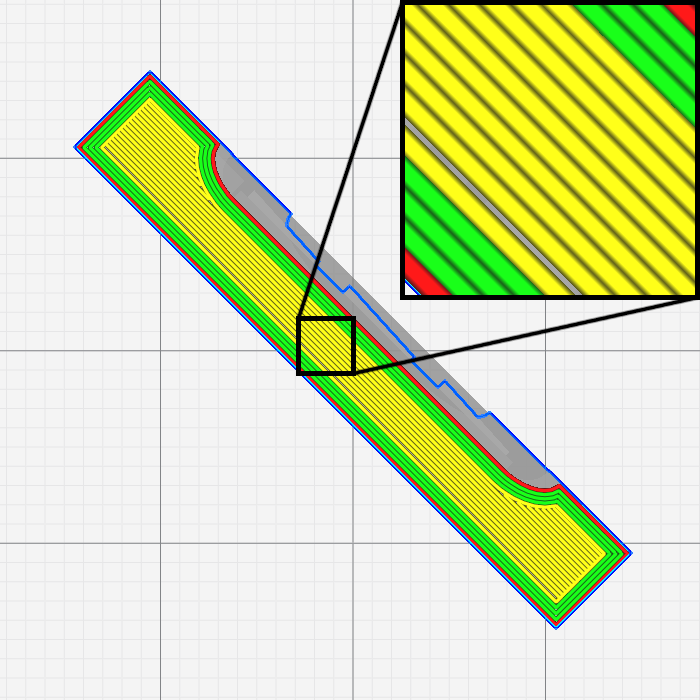
\includegraphics[width=\textwidth]{\Figures/Moules/coupe_diag_zoom.png}
    \end{subfigure}
    \begin{subfigure}[b]{0.30\textwidth}
       \centering \caption{
            \label{fig:print:shield}
            Enceinte pare-brise autour d'un tampon
            }
       \centering 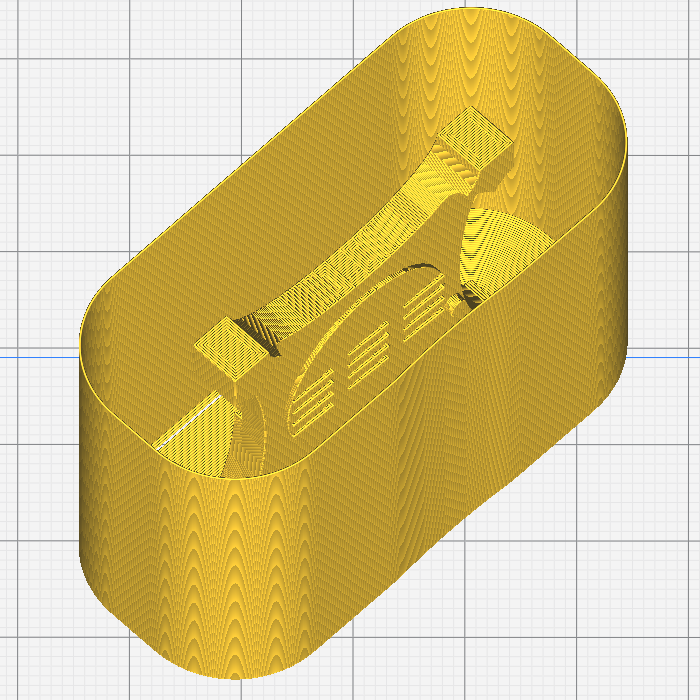
\includegraphics[width=\textwidth]{\Figures/Moules/shield.png}
    \end{subfigure}
    \caption{
        \label{fig:print}
        Exemple de solutions permettant l'amélioration de la qualité d'impression.
        \newline
        Comme on peut le voir dans les encarts de (a) et (b), positionner le moule dans l'axe d'impression permet d'augmenter la longueurs des d'allers\hyp{}retours, ce qui reduit les stress mécaniques et limite les risques de ruptures de la pièce en impression.
        L'impression d'une enceinte pare-brise  simultanément à l'impression des tampons(c) empêche les différences thermiques pouvant affecter la qualité d'impression.
    }
\end{figure}

%%
%
En couplant ces différentes optimisations, j'ai pu réaliser des impressions précises, tout en réduisant les taux d'échec d'impression.

\end{document}
